%========================
% Theme
%========================
\documentclass[8pt]{beamer}
\setbeamersize{text margin left=10mm,text margin right=10mm} 
\usetheme[progressbar=frametitle]{metropolis}
\usepackage{appendixnumberbeamer} % handles appendix slide numbering

%========================
% Packages: Icons and Tables
%========================
\usepackage{booktabs}        % professional tables
\usepackage[scale=1]{ccicons} % Creative Commons icons

%========================
% Packages: Plots and TikZ
%========================
\usepackage{pgfplots}
\usepgfplotslibrary{dateplot}

\usepackage{tikz}
\usetikzlibrary{positioning}

%========================
% Packages: Algorithms
%========================
\usepackage{algorithm}
\usepackage{algpseudocode}

%========================
% Packages: Math
%========================
\usepackage{amsmath,amsfonts,amsthm,amssymb}
\newtheorem{prop}{Proposition}

%========================
% Custom commands
%========================
\usepackage{xspace}
\newcommand{\themename}{\textbf{\textsc{metropolis}}\xspace}

%========================
% Custom footline
%========================
\setbeamertemplate{footline}
{%
  \leavevmode%
  \hbox{%
  \begin{beamercolorbox}[wd=.35\paperwidth,ht=2.5ex,dp=1.5ex,center]{author in head/foot}%
    \usebeamerfont{author in head/foot}\insertshortauthor
  \end{beamercolorbox}%
  \begin{beamercolorbox}[wd=.3\paperwidth,ht=2.5ex,dp=1ex,center]{title in head/foot}%
    \usebeamerfont{title in head/foot}\insertshorttitle
  \end{beamercolorbox}%
  \begin{beamercolorbox}[wd=.3\paperwidth,ht=2.5ex,dp=1ex,right]{date in head/foot}%
    \usebeamerfont{date in head/foot}\insertframenumber{} / \inserttotalframenumber
  \end{beamercolorbox}}%
  \vskip0pt%
}

%========================
% Remove default navigation symbols
%========================
\setbeamertemplate{navigation symbols}{}

\usepackage{pgf,pgfarrows,pgfnodes,pgfautomata,pgfheaps,pgfshade}
\usepackage{hyperref}
\usepackage{listings}
\usepackage{color}

\lstset{language=R,
    basicstyle=\small\ttfamily,
    stringstyle=\color{DarkGreen},
    otherkeywords={0,1,2,3,4,5,6,7,8,9},
    morekeywords={TRUE,FALSE},
    deletekeywords={data,frame,length,as,character},
    keywordstyle=\color{blue},
    commentstyle=\color{DarkGreen},
}

\usepackage{xcolor}

\lstset{
    language=Python,
    basicstyle=\ttfamily\small,
    keywordstyle=\color{blue},
    commentstyle=\color{gray},
    stringstyle=\color{red},
    breaklines=true,
    numbers=left,
    numberstyle=\tiny
}



%%%%%%%%%%%%%%%%%%%%%%%%%%%%%%%%%%%%%%%%%%%%%%%%%%%%%%%%%%%%%%%%%%%%
%%%%%%%%%%%%%%%%%%%%%%%%%%%%%%%%%%%%%%%%%%%%%%%%%%%%%%%%%%%%%%%%%%%%
% AQUI SE DEFINEN LAS IMAGENES PARA UTILIZAR DESPUES
%\pgfdeclareimage[interpolate=true, height=7cm,width=16cm]{halton-points}{halton-points}
%\pgfdeclareimage[interpolate=true, height=3cm, width =4cm]
%{serie-petroleo-reducido}{serie-petroleo-reducido}
%\pgfdeclareimage[interpolate=true, height=3cm, width =4cm]{rectangle-triangle}{rectangle-triangle}
%\pgfdeclareimage[interpolate=true, height=3cm, width =4cm]{any-angle}{any-angle}
%\pgfdeclareimage[interpolate=true, height=3cm, width =4cm]{Pythagoras}{Pythagoras}


\title{Chapter 1 - Random Number Generation}
\subtitle{Transformation of Random Variables. Box Muller Transformation.}
\author{Prof. Alex Alvarez, Ali Raisolsadat}
\institute{School of Mathematical and Computational Sciences \\ University of Prince Edward Island}
\date{} % leave empty or add \today
%\title[Stat 4110]{Stat 4110 Statistical Simulation}
%\subtitle{}
%\author[University of Prince Edward Island]{School of Mathematical and Computational Sciences \\ University of Prince Edward Island}

%========================
% Begin document
%========================
\begin{document}

%-------------------
% Title frame
%-------------------
\maketitle

%-------------------
% Slide 1: Transformation of random variables
%-------------------
\begin{frame}{Transformation of Random Variables}
The inverse transform method is an example of how to transform a uniform random variable into a random variable with a different distribution. 

\vspace{2mm}

This is just one example of a possible transformation of random variables. 

\vspace{2mm}

There are more complicated transformations of random variables
that could be useful in some cases.
\end{frame}

%-------------------
% Slide 2: Transformation of Random Vectors
%-------------------
\begin{frame}{Transformation of Random Vectors}
In some cases it might be convenient to transform a whole random vector from $\mathbb{R}^d$ into a new random vector from $\mathbb{R}^d$
in order to get random numbers/vectors with a desired distribution.

\vspace{2mm}

Perhaps the most noticeable example of this is the \textbf{Box-Muller transform} for the generation of normal random variables.

\vspace{2mm}

This comes as an application of a very general result from the textbook (\textbf{Theorem 1.34}).
\end{frame}

%-------------------
% Slide 3: Box-Muller Transform Algorithm
%-------------------
\begin{frame}{Box-Muller Transform Algorithm}
\alert{Algorithm}  

\begin{enumerate}
	\item Generate $\Theta \sim U[0,2\pi]$ and $U\sim U[0,1]$ independently
	\item Compute $R=\sqrt{-2\ln(U)}$
	\item Compute $(X,Y)=(R \cos \Theta  , R \sin \Theta)$
	\item Return $(X,Y)$
\end{enumerate}
The random variables $X$, $Y$ are independent, standard normal random variables.
\end{frame}

%-------------------
% Slide 4: Box-Muller Transform Remarks
%-------------------
\begin{frame}{Box-Muller Transform}
\textbf{Remarks}: 

\begin{itemize}
	\item Unfortunately, as we have discussed earlier in the course (see slides corresponding to the Inverse transform method) \textbf{we cannot transform a single uniformly distributed random variable into a single normal random variable easily}
	\item However, with the Box-Muller algorithm \textbf{we can transform two independent, uniformly distributed random variables into two independent standard normal random variables.}
	\item This type of transformations (from $\mathbb{R}^d$ to $\mathbb{R}^d$) are not very common and the Box-Muller algorithm is a very notable exception.
	\item Some textbooks also refer to this method as the \textbf{polar method}.
\end{itemize}
\end{frame}

%-------------------
% Slide 5: Box-Muller Transform Example
%-------------------
\begin{frame}[fragile]{Box-Muller Transform Example}
\alert{Code}
\vspace{2mm}

\begin{columns}
\column{0.45\textwidth}
\textbf{R Code}
\begin{lstlisting}
n <- 1000
m <- n/2
X <- vector()
R <- vector()
U <- runif(m, min=0, max =1)
Theta <- 
  runif(m, min=0, max = 2*pi) 

for (i in c(1:m)) {
  R[i] <- sqrt(-2*log(U[i])) 
  X[2*i-1]<- R[i]*cos(Theta[i]) 
  X[2*i]<- R[i]*sin(Theta[i])
} 

hist(X)
\end{lstlisting}

\column{0.55\textwidth}
\textbf{Python Code}

\begin{lstlisting}
import numpy as np
import matplotlib.pyplot as plt

n = 1000
m = n // 2
X = np.zeros(n)
R = np.zeros(m)
U = np.random.uniform(0, 1, m)
Theta = np.random.uniform(0, 2*np.pi, m)

for i in range(m):
    R[i] = np.sqrt(-2 * np.log(U[i]))
    X[2*i] = R[i] * np.cos(Theta[i])
    X[2*i+1] = R[i] * np.sin(Theta[i])

plt.hist(X, bins=30)
plt.show()
\end{lstlisting}
\end{columns}
\end{frame}

%-------------------
% Slide 6: Box-Muller Transform Example Plot
%-------------------
\begin{frame}{Visualizing the Uniform Sample Under a PDF}
\begin{center}
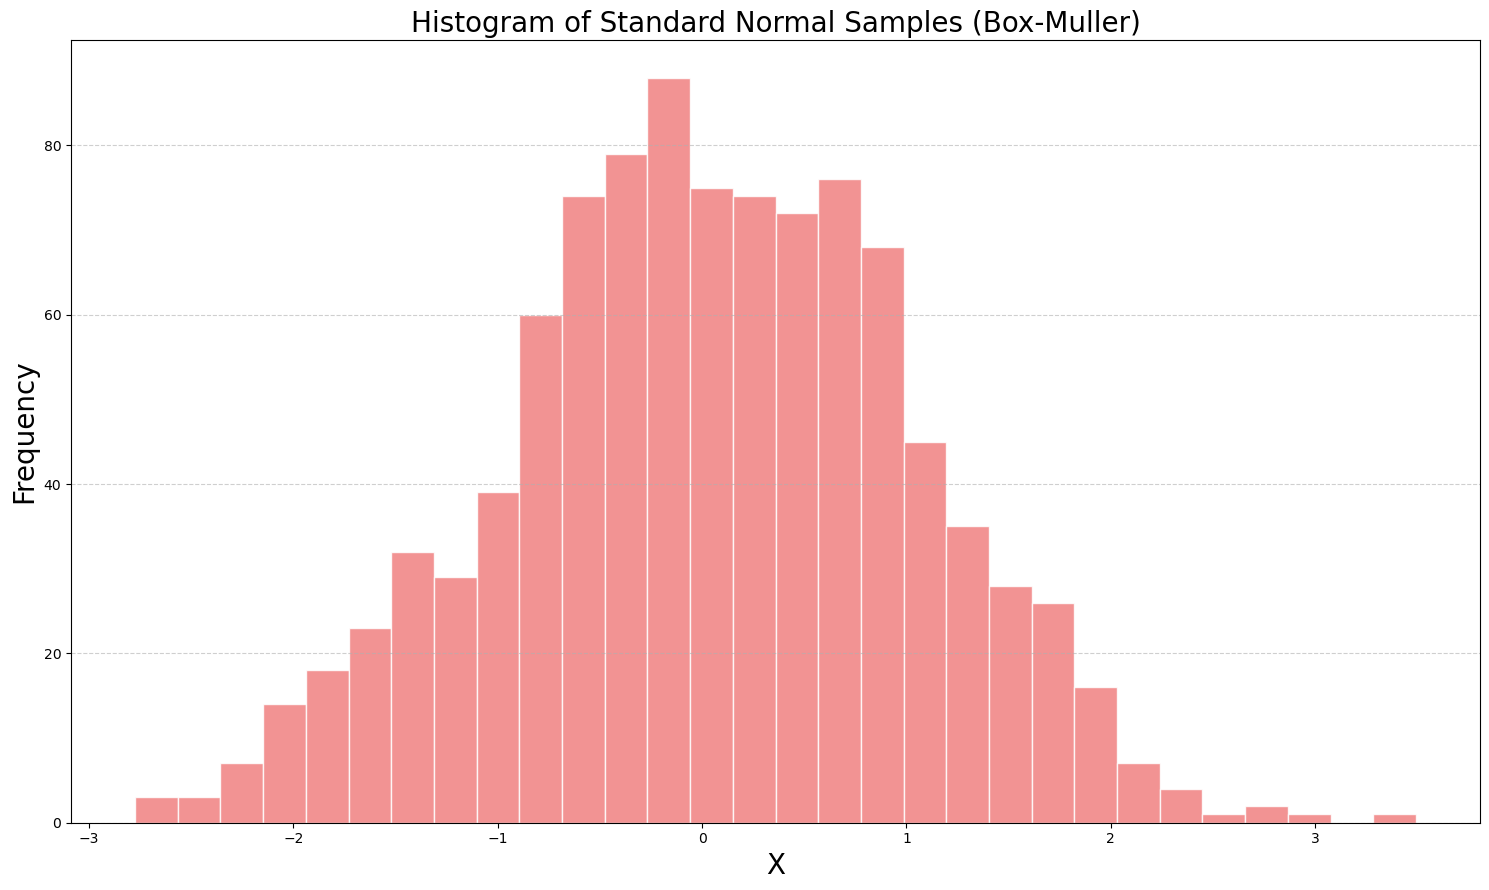
\includegraphics[width=\textwidth]{chapter1-part6-plot1.png}
\end{center}
\end{frame}




\end{document}